\documentclass[]{article}
\usepackage[a4paper, total={6in, 8in}]{geometry}
\usepackage[english]{babel}	
\usepackage[utf8]{inputenc} % Umlaute
\usepackage{amssymb}
\usepackage{amsmath} 
\usepackage{fancyhdr}
\usepackage{fancyvrb} % Für regex Umgebung
\usepackage{multicol} % Mehrere Spalten
\usepackage{graphicx} % bilder
\usepackage[table]{xcolor}
\usepackage{hyperref}
\pagestyle{fancy}
\fancyhf{} %clears the header and footer
\rhead{Professor Robert Feldmann (lectures) \\ Dr. Darren Reed (exercise classes) \\ Dimakopoulos Vasileios (TA) \\ Elia Cenci (TA)}
\lhead{Universität Zürich \\ Institute for Computational Science \\ Spring Semester 2021 \\ Final Exam ESC403 - Dave Linder}
\fancyfoot[C]{\thepage}


\title{\textbf{\normalsize INTRODUCTION TO DATA SCIENCE \\ \Large FINAL EXAM 2021}}
\author{Solutions from David Linder}

\begin{document}
	\maketitle
	\thispagestyle{fancy}
	This are my solutions to the final exam 2021 in introduction to data science. All the computations and the code as well as the data and plots and also this document can be found in the git-repository: \href{https://github.com/massstab/ESC403_exam.git}{https://github.com/massstab/ESC403\_exam.git}. I included also the .csv files asked for in the folder \texttt{report/data/}.
	\section{Time Series}
	\subsection{}
	To be considered stationary a time series should have the following properties:
	\begin{itemize}
		\item The mean $E[X_t]$ is the same for all times $t$.
		\item The variance $Var[X_t]$ is the same for all times $t$.
		\item The covariance between $X_t$ and $X_{t-1}$ is the same for all $t, n$.
	\end{itemize}
	That means we want
	\begin{itemize}
		\item no obvious trends.
		\item constant variance with time.
		\item constant autocorrelation structure over time.
		\item no periodic fluctuations (no seasonality).
	\end{itemize}
	I found some examples \href{https://otexts.com/fpp2/stationarity.html}{here}: In figure \ref{fig:time_series} we see that most of the series are non-stationary except series (b) and (g). In series (g) there are cycles but they are not periodic. 
	\begin{figure}
		\centering
		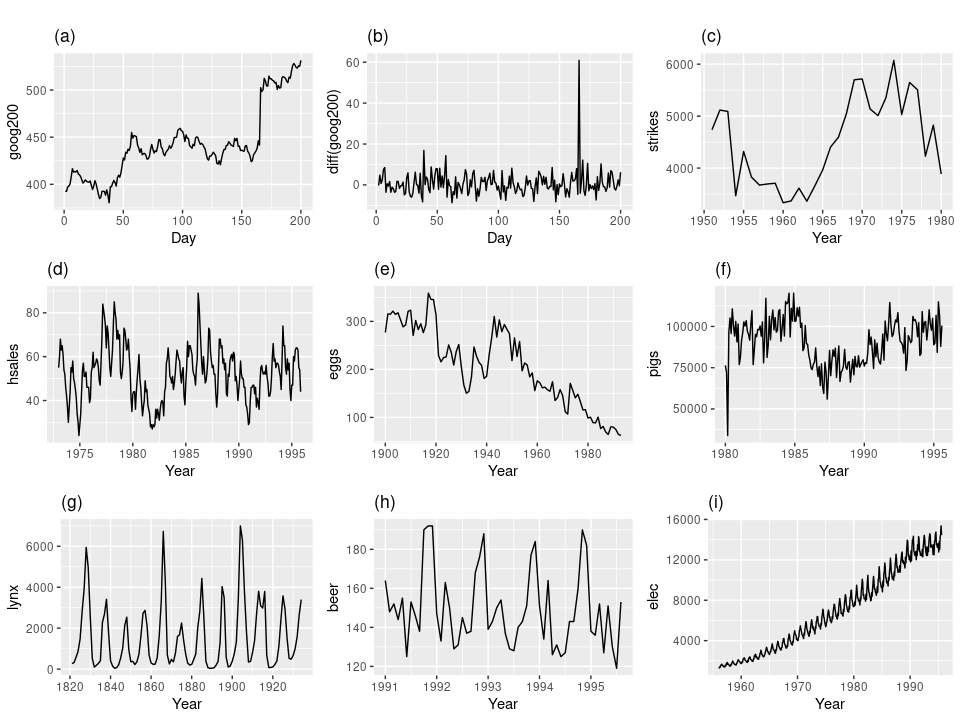
\includegraphics[width=0.8\textwidth]{images/time_series.png}
		\caption{(a) Google stock price for 200 consecutive days; (b) Daily change in the Google stock price for 200 consecutive days; (c) Annual number of strikes in the US; (d) Monthly sales of new one-family houses sold in the US; (e) Annual price of a dozen eggs in the US (constant dollars); (f) Monthly total of pigs slaughtered in Victoria, Australia; (g) Annual total of lynx trapped in the McKenzie River district of north-west Canada; (h) Monthly Australian beer production; (i) Monthly Australian electricity production.}
		\label{fig:time_series}
	\end{figure}
	
	\subsection{}
	
	\begin{itemize}
		\item By looking at the data we can clearly see that this time series is not stationary. After log transformed the $X$-data we can see in figure \ref{fig:rollingmean} 
		\begin{figure}
			\centering
			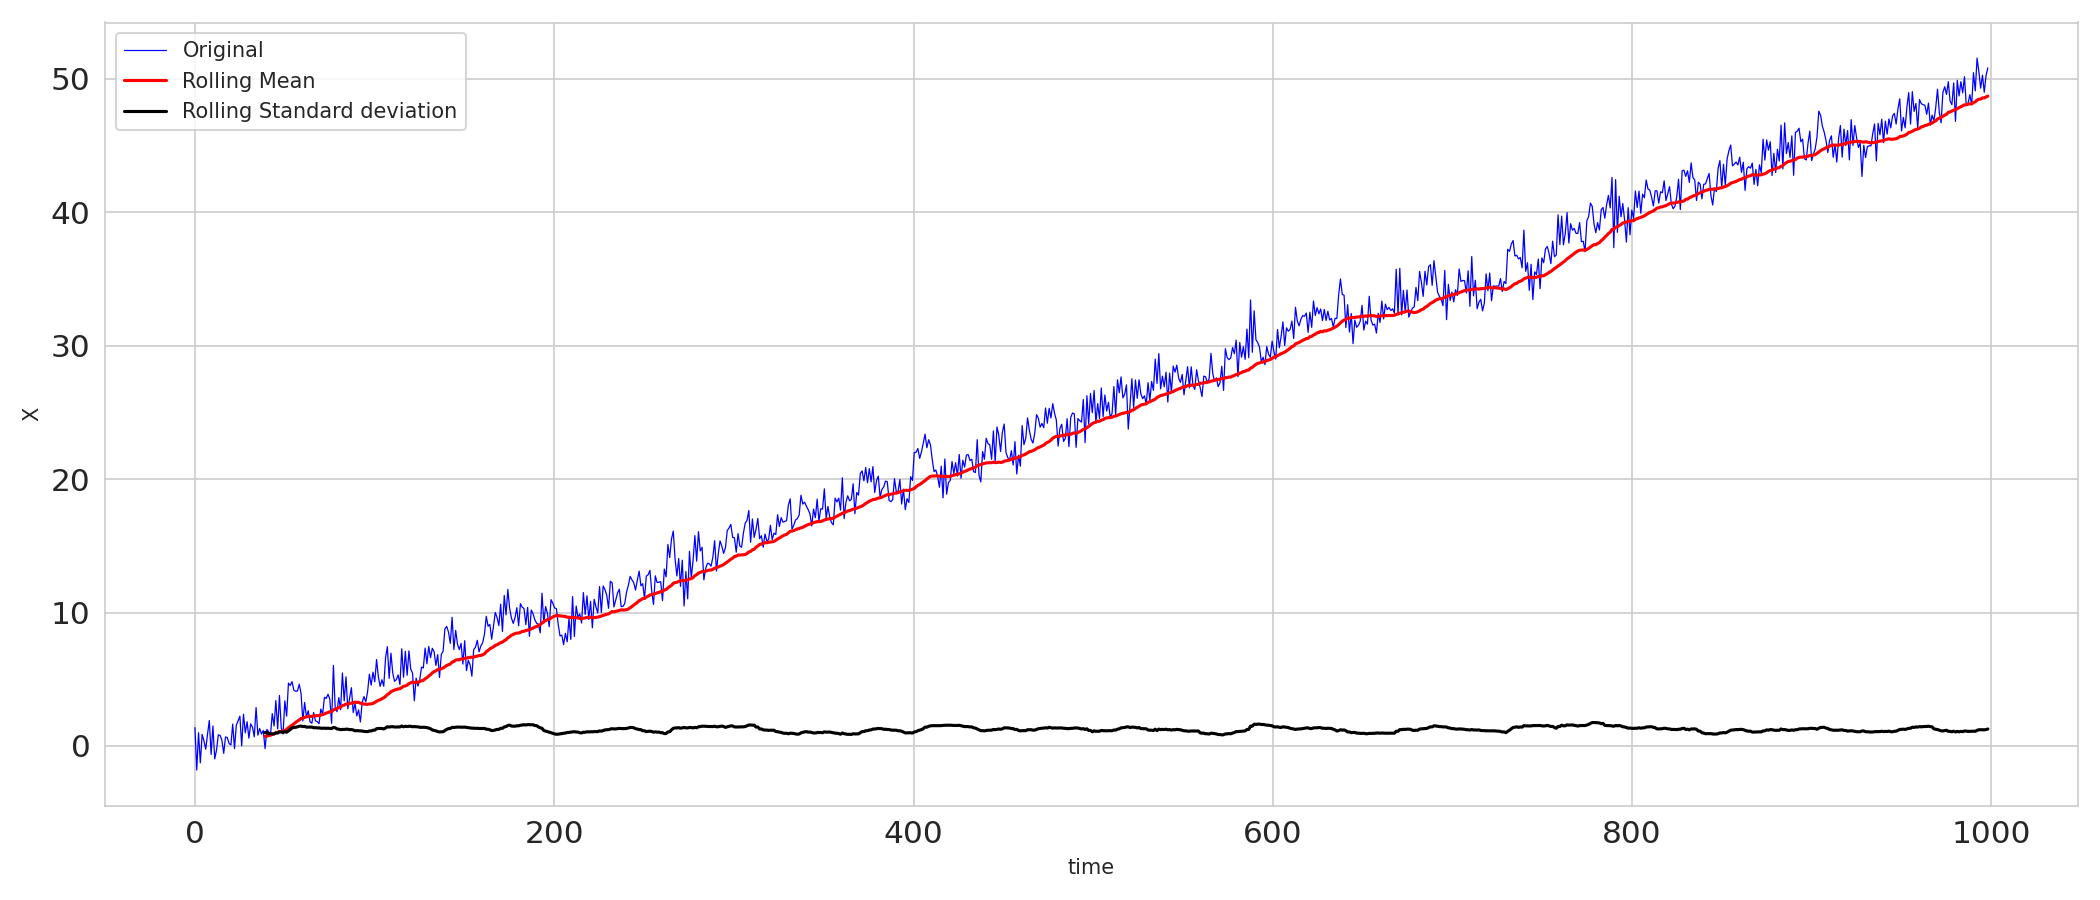
\includegraphics[width=1\textwidth]{images/ts_log.png}
			\caption{The time series after a log-transformation. This series is clearly not stationary. The mean increases over time.}
			\label{fig:rollingmean}
		\end{figure}
		that although the standard deviation has a small variation the mean increases over time. Also the results of the Dickey-Fuller test is that we can not reject $H_0$ (TS is non-stationary) because the test statistic value is not less than any critical value. Here is the data in detail: 
		\begin{center}
			\begin{tabular}{|l|r|}
				\hline Test Statistic & $-0.2312$ \\
				\hline p-value & $0.9347$ \\
				\hline Lags & $22.0000$ \\
				\hline Observations & $975.0000$ \\
				\hline Critical Value $(1 \%)$ & $-3.4371$ \\
				\hline Critical Value $(5 \%)$ & $-2.8645$ \\
				\hline Critical Value $(10 \%)$ & $-2.5684$ \\
				\hline
			\end{tabular}
			\label{tab:dickey}
		\end{center}
		I will use the moving average smoothing method which we used in the exercise class to eliminate the trend. First i calculated the rolling mean with the pandas function and then subtracted this from the original series (code: \texttt{timeseries/Q1.2.py}). Then i dropped all the nan values that resulted from averaging over the time window (i tried out different sizes of that window and ended up with a value of 40). To remove seasonality i applied differencing. In figure \ref{fig:rollingmean_diff} we see the result and that we eliminated the trend.
		\begin{figure}
			\centering
			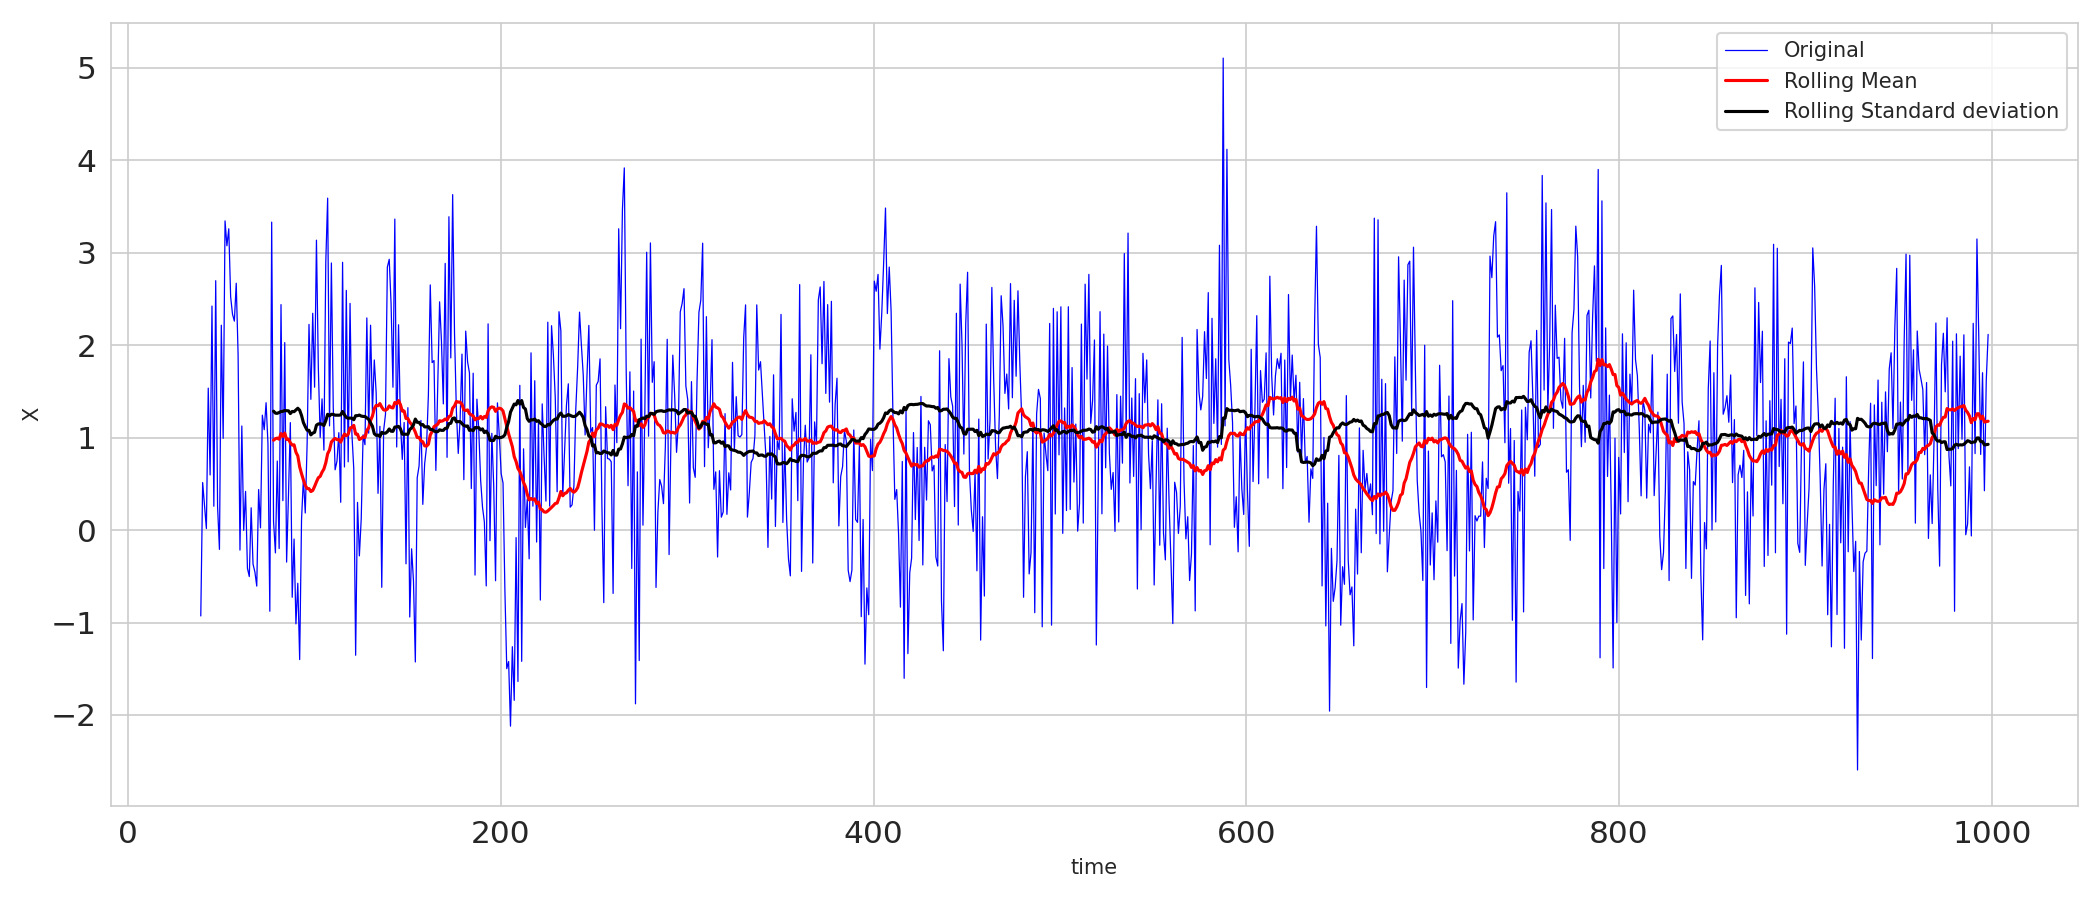
\includegraphics[width=1\textwidth]{images/ts_log_moving_avg_diff.png}
			\caption{The result from smoothing and differencing. We can now consider this as a stationary time series.}
			\label{fig:rollingmean_diff}
		\end{figure}
		Let's take a look at the test statistics:
		\begin{center}
			\begin{tabular}{|l|r|}
				\hline Test Statistic & $-10.7860$ \\
				\hline p-value & $0.0000$ \\
				\hline Lags & $1.0000$ \\
				\hline Observations & $937.0000$ \\
				\hline Critical Value $(1 \%)$ & $-3.4373$ \\
				\hline Critical Value $(5 \%)$ & $-2.8646$ \\
				\hline Critical Value $(10 \%)$ & $-2.5684$ \\
				\hline
			\end{tabular}
		\end{center}
		The value is lower than all the critical values. Therefore we can say at least with 99\% confidence this is now a stationary time-series.
		

		\item For answering this question we need to find the p-value. For this value to find we look at the plot of the partial autocorrelation function (PACF). From figure \ref{fig:pacf} we find a p-value of 3. That means that 3 values of at prior times are expected to directly affect a given current value of the time series.
		\begin{figure}
			\centering
			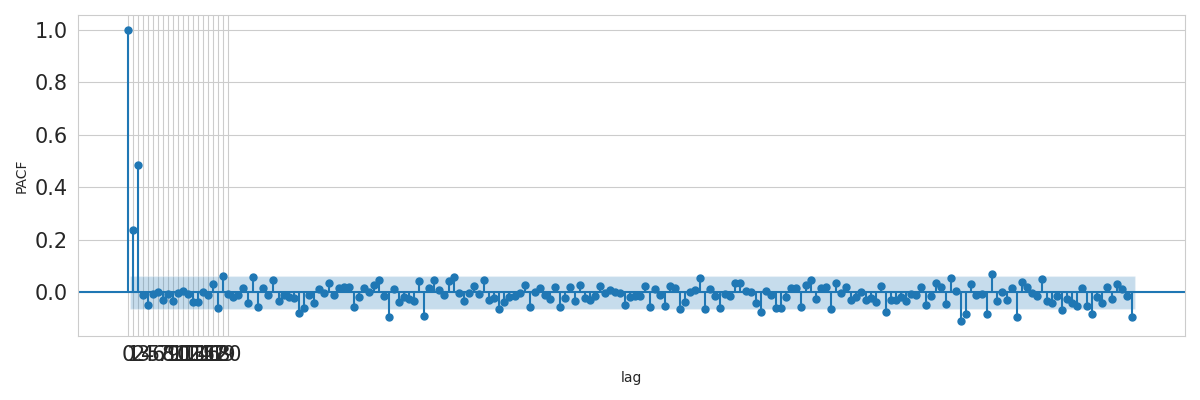
\includegraphics[width=1\textwidth]{images/partialautocorrelation.png}
			\caption{Plot of the partial autocorrelation function. The x-axis are the lags. One can see that the first time the PACF crosses the confidence interval (blue) is at lag 3.}
			\label{fig:pacf}
		\end{figure}
		\item To find which ARIMA model would be appropriate we look at the autocorrelation function in. We clearly can see that the function decays to zero while alternating between + and -. This seems to be an AR model (for which we already identified the p-value as 3). Maybe one could also try a mixed AR and MA model. For this i also identified the q value. The function crosses the confidence interval at lag 7 $\implies q=7$. 
		\begin{figure}
			\centering
			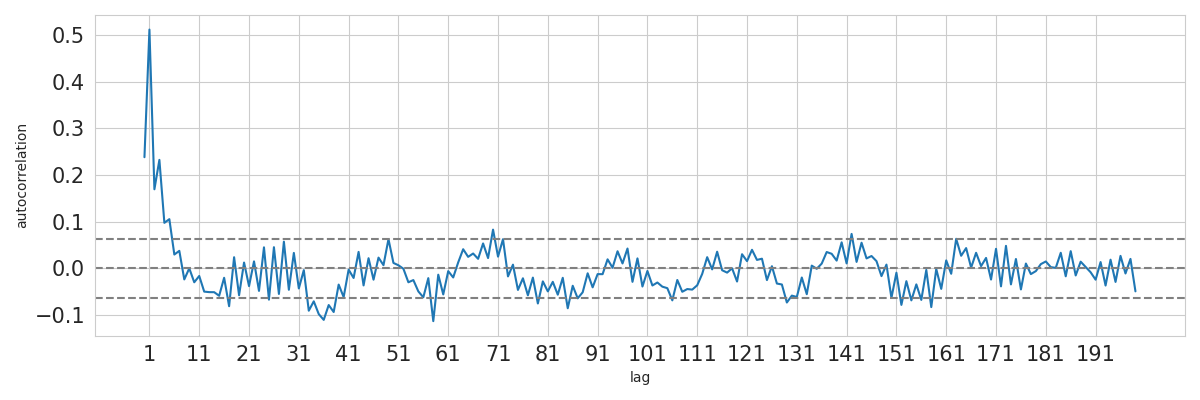
\includegraphics[width=1\textwidth]{images/autocorrelation_identification.png}
			\caption{The autocorrelation function to identify the ARIMA model.}
			\label{fig:acf}
		\end{figure}
	\end{itemize}
	
	\subsection{}
	\begin{itemize}
		\item In figure \ref{fig:rollingmean_B} we see the mean increasing over time. Here the results from the test statistic:
		\begin{center}
			\begin{tabular}{|l|r|}
				\hline Test Statistic & $-0.5905$ \\
				\hline p-value & $0.8730$ \\
				\hline Lags & $23.0000$ \\
				\hline Observations & $2031.0000$ \\
				\hline Critical Value $(1 \%)$ & $-3.4335$ \\
				\hline Critical Value $(5 \%)$ & $-2.8629$ \\
				\hline Critical Value $(10 \%)$ & $-2.5675$ \\
				\hline
			\end{tabular}
		\end{center}
		\begin{figure}
			\centering
			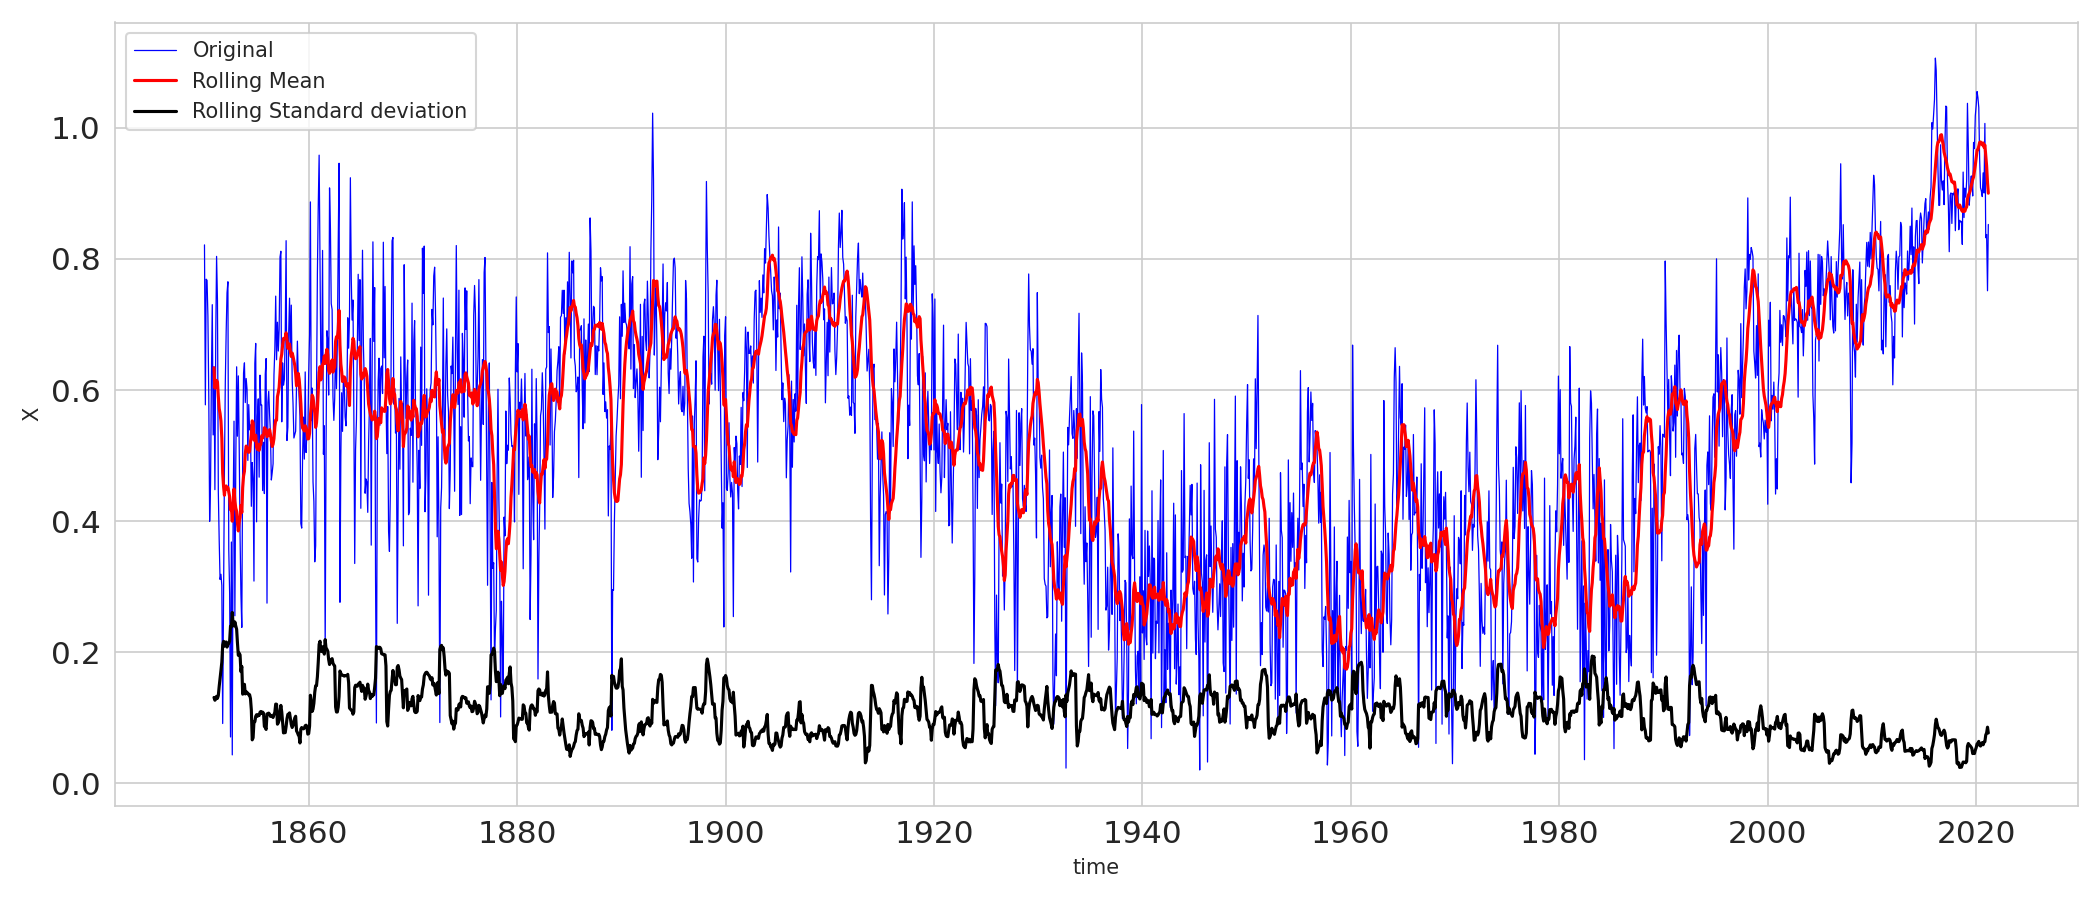
\includegraphics[width=1\textwidth]{images/ts_moving_avg_B.png}
			\caption{Average temperature anomaly raw data.}
			\label{fig:rollingmean_B}
		\end{figure}
		After differencing the time-series looks stationary as we ca see in figure \ref{fig:rollingmean_diff_B}. Let's support that with the statistics:
		\begin{center}
			\begin{tabular}{|l|r|}
				\hline Test Statistic & $-15.7773$ \\
				\hline p-value & $0.0000$ \\
				\hline Lags & $22.0000$ \\
				\hline Observations & $2031.0000$ \\
				\hline Critical Value $(1 \%)$ & $-3.4335$ \\
				\hline Critical Value $(5 \%)$ & $-2.8629$ \\
				\hline Critical Value $(10 \%)$ & $-2.5675$ \\
				\hline
			\end{tabular}
		\end{center}
		The test statistic value is clearly under the critical value of 1\% therefore we can say whit at least 99\% certainty that this is now a stationary time series.
		\begin{figure}
			\centering
			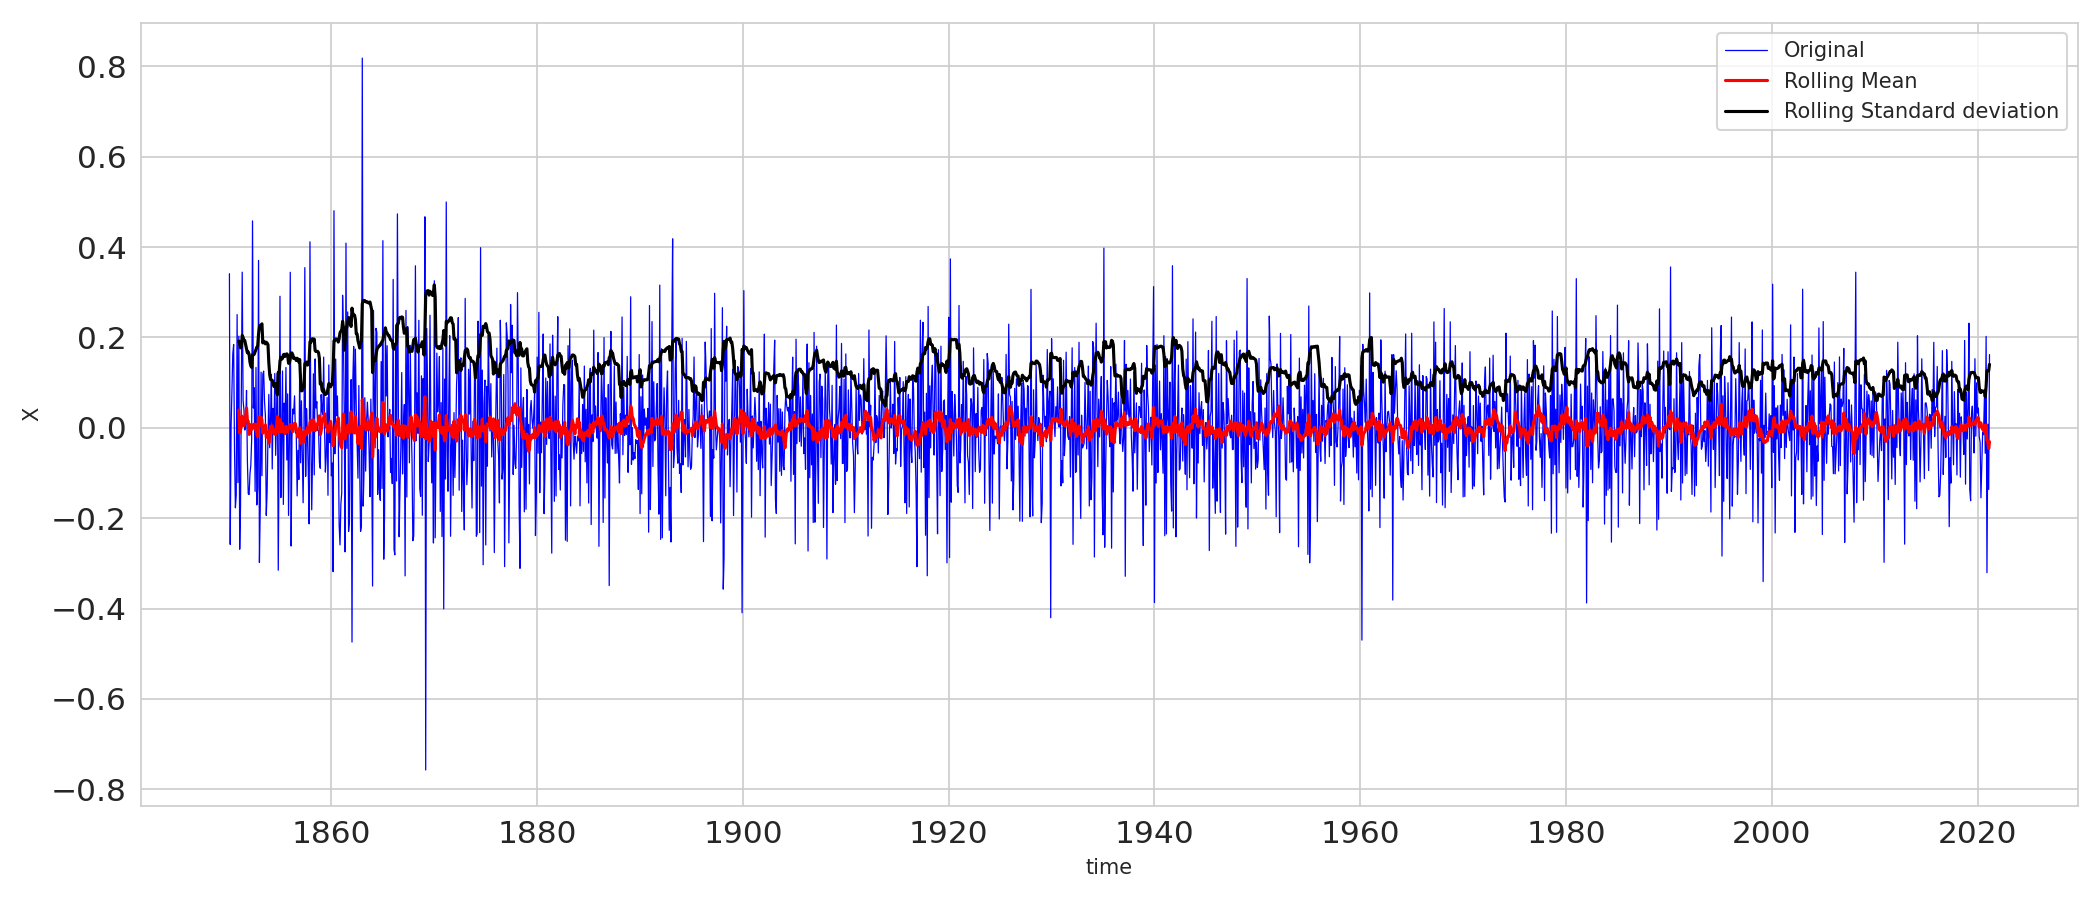
\includegraphics[width=1\textwidth]{images/ts_moving_avg_diff_B.png}
			\caption{Average temperature anomaly after differencing.}
			\label{fig:rollingmean_diff_B}
		\end{figure}
		To find the p and q we look at the ACF and PACF in figure \ref{fig:acf_B} and \ref{fig:pacf_B} respectively.
		\begin{figure}
			\centering
			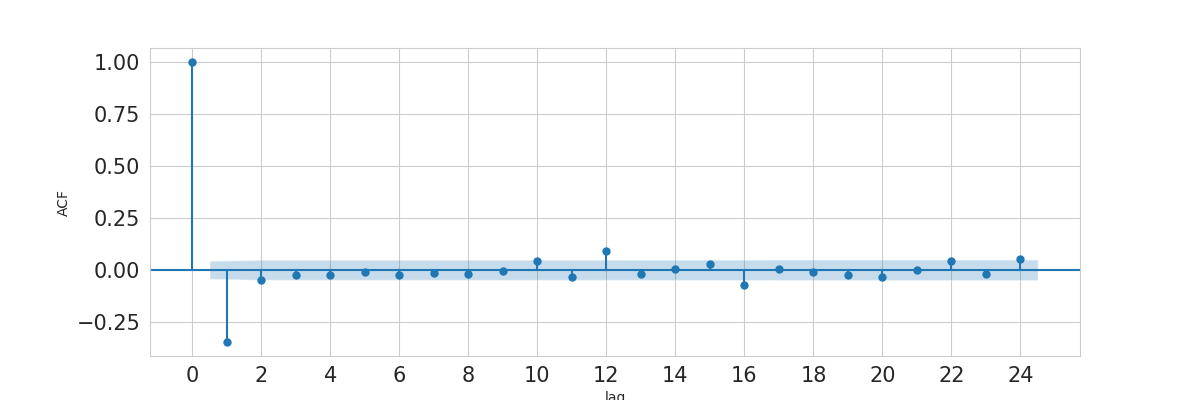
\includegraphics[width=0.8\textwidth]{images/autocorrelation_B.png}
			\caption{The autocorrelation function. One can see that the first time the ACF crosses the confidence interval (blue) is at lag 2.}
			\label{fig:acf_B}
		\end{figure}
		\begin{figure}
			\centering
			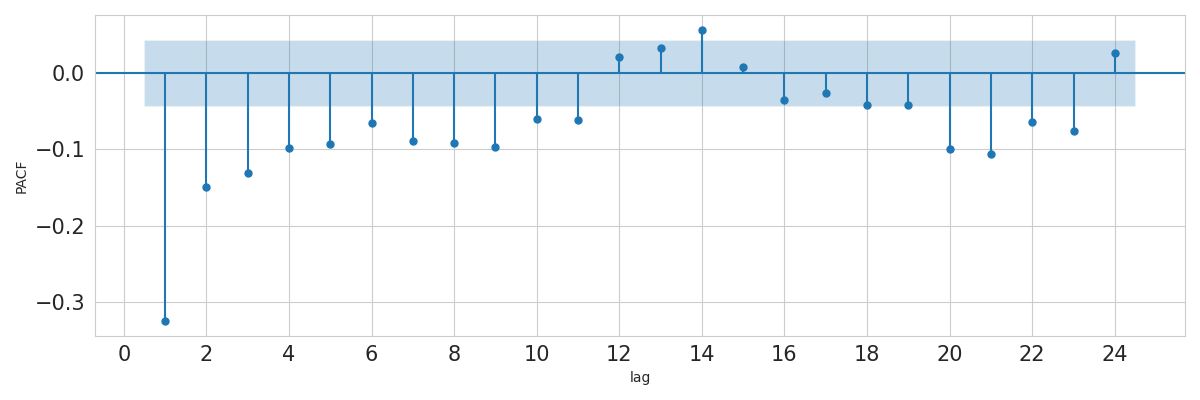
\includegraphics[width=0.8\textwidth]{images/partialautocorrelation_B.png}
			\caption{The partial autocorrelation function. One can see that the first time the PACF crosses the confidence interval (blue) is at lag 12.}
			\label{fig:pacf_B}
		\end{figure}
		And we find for $p=12$ and $q=2$.

		We use a KDE to see the residuals and its variance. In figure \ref{fig:res_dens} we can see that the mean of the residuals is near zero with a good uniform variance. That means we can use the model to predict future values.
		\begin{figure}
			\centering
			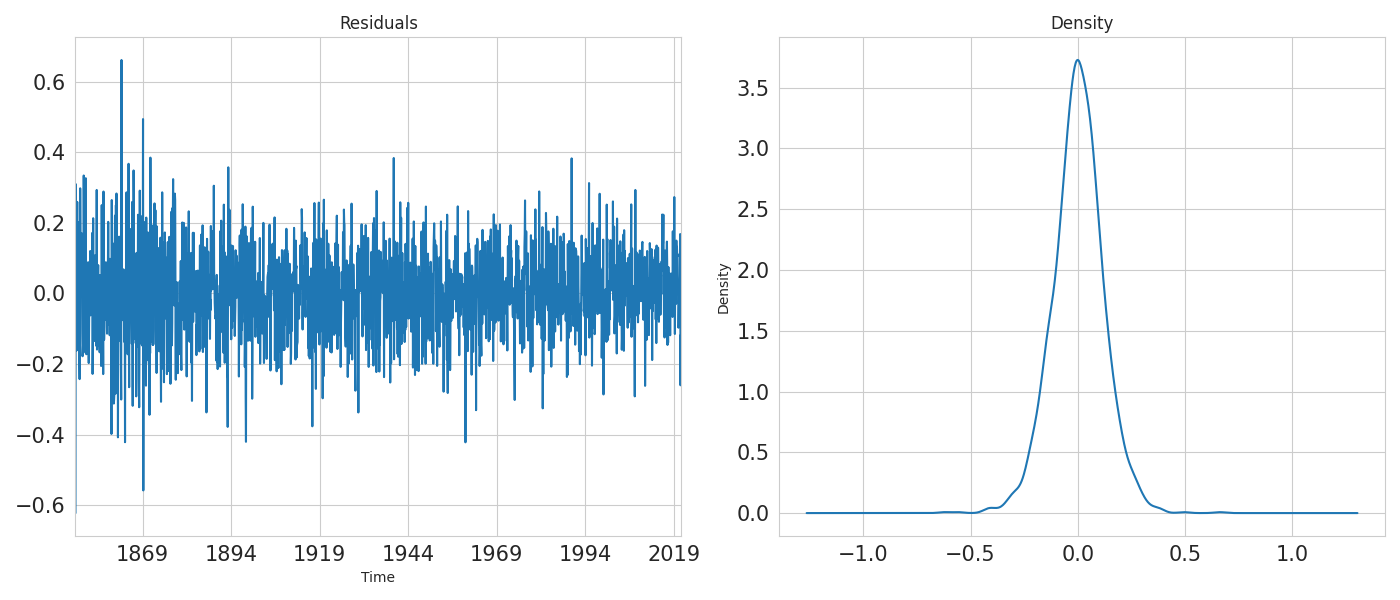
\includegraphics[width=1\textwidth]{images/res_dens.png}
			\caption{Residuals and density.}
			\label{fig:res_dens}
		\end{figure}
				
		
		\item Here we try to give a prediction for the average temperature anomaly from the years 2010-2021. In figure \ref{fig:forecast_2010-2021} we see in orange the measured values and in blue the prediction with the ARIMA model.
		The resulted RMSE of only 0.1188 seems a bit low to me.
		\begin{figure}
			\centering
			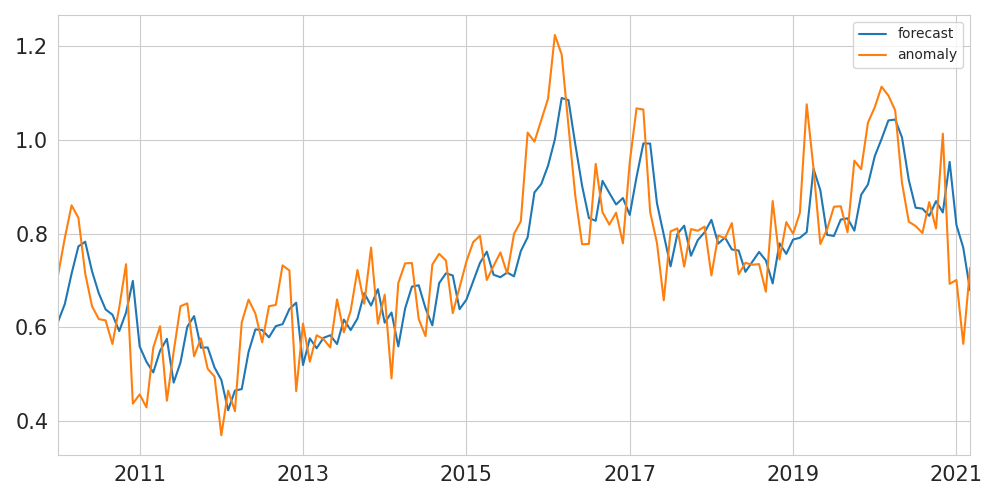
\includegraphics[width=0.7\textwidth]{images/forecast_2010-2021.png}
			\caption{Forecast 2010 - 2021}
			\label{fig:forecast_2010-2021}
		\end{figure}
		\begin{figure}
			\centering
			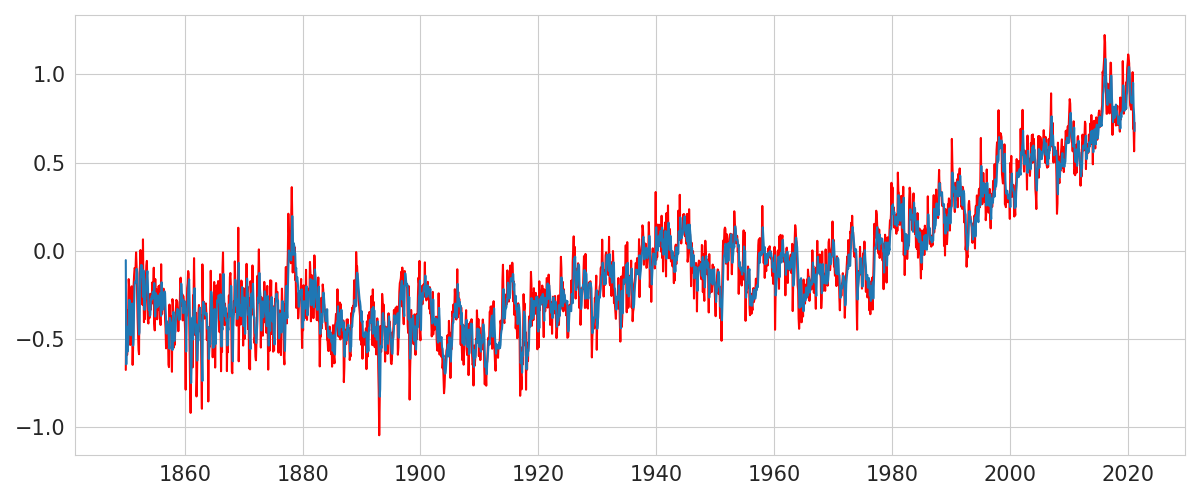
\includegraphics[width=0.7\textwidth]{images/forecast_2010-2021_RMSE.png}
			\caption{Forecast 2010 - 2021. This resulted in a RMSE of 0.1188.}
			\label{fig:forecast_2010-2021_RMSE}
		\end{figure}
		\item I tried a lot of different models and values for p ad q. But all gave some very fast decaying solution for my prediction like in figure 
		\begin{figure}
			\centering
			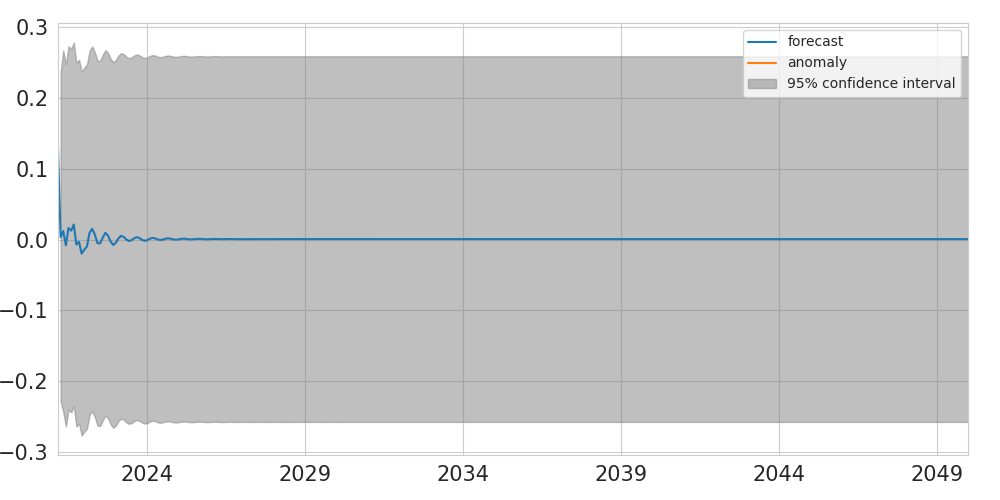
\includegraphics[width=0.7\textwidth]{images/forecast_2021-2050.png}
			\caption{Forecast 2021 - 2050. The model always ended up giving me decaying results. Doesn't matter what parameters of the ARIMA model i tweak'd.}
			\label{fig:forecast_2021-2050}
		\end{figure}
	\end{itemize}
	\section{Image classification}
	\subsection{Image classification}
	If better means higher accuracy then i would choose a CNN for image classification. RF performs well on categorical data while a CNN handles numerical input very well. Here we have pixels with numerical values between 0 and 255. We can also tune more parameters in a CNN like kind/number of layers, epochs and learning rate. Also different activation functions for the neurons can be chosen. Finally a CNN learns how to apply a filter to an input during training such that certain features in the image can be recognized. A RF can not take advantage of such structures in images.
	
	On the other hand a CNN needs a lot of data to perform well. I don't know exactly if our dataset is large enough but if i compare with other models they used hundred thousands or even millions of images to train a CNN.

	\subsection{Classification performance}
	\begin{itemize}
		\item Accuracy CNN: 99.1\%, that means the error rate was 1\%. It misclassified 10/1000 images from my test set.
		\item Accuracy RF: 99.6\%, that means the error rate was 0.4\%. It misclassified 5/1000 images from my test set.
		\item Both models performed surprisingly good. I checked many times if i excluded any test data from the training. No model performed significantly better.
		\item Both models agreed in all images only the CNN misclassified image 001212.jpg where it predicted the class 'headCT' instead of 'Hand'. As far as i can tell the RF made no prediction error on the unlabeled dataset. The predictions with the images can be found in figure \ref{fig:pred_img} in the appendix.
		I included the corresponding files in the folder \texttt{report/data} in the repository (\texttt{predictions\_cnn.csv}, \texttt{predictions\_rf.csv}).
	\end{itemize}
	
	\subsection{Hyper parameter tuning}
	\begin{itemize}
		\item For the random forest i pretty much left the default parameters. I played around with the depth of the tree (max\_depth) and the number of trees in the forest (n\_estimators). Nothing gave me significant improvement. The only thing i did was switching off bootstrapping.
		\item The CNN i started from an older task i did with image recognition. For the optimizer i choose adam with a learning rate of 0.001. I played around with number of layers and filters in the Conv2D layers. For performance reason i did a pooling layer at the end of two consecutive convolutional layers. I also played around with the kernel size and different activation function such as relu and sigmoid. After a flattening layer i applied a dense layer followed by a dropout layer (quiet high 50\%) and a dense layer at the end with a softmax of 6 unit (one per class) which gave me the probabilities for each class. A detailed plot of the model built with keras can be found in the appendiy in figure \ref{fig:model_cnn}. 
	\end{itemize}
	
	\subsection{Interpretation of model performance}
	For the training and validation accuracy and loss i made a plot in figure \ref{fig:history}. The evaluation of the random forest model i did with the sklearn integrated method \texttt{precision\_recall\_fscore\_support()}. This module provides information about precision, recall and f-score. I couldn't do a out-of-bag (OOB) error estimation because i turned bootstrapping of. All this can be seen in the script \texttt{classification/Q2.py}. I couldn't see much under- or overfitting on the models or bias. But to prevent overfitting in random forest i would probably turn on bootstrapping or growing a larger forest.
	
	To avoid bias i would look at the bias-variance trade-off. As we learned in class, more flexible methods tends to have lower bias but higher variance and more restrictive methods tend to have lower variance but higher bias. Then i would choose the mothod with the right amount of flexibility to minimize test error (via cross validation). 
	\begin{figure}
		\centering
		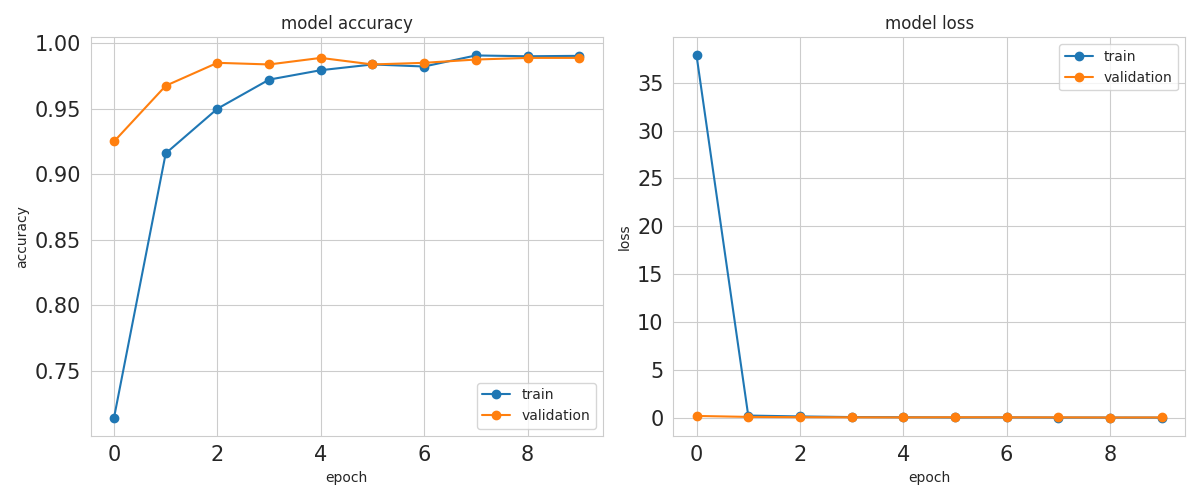
\includegraphics[width=1\textwidth]{images/history.png}
		\caption{CNN training and validation accuracy and loss in the training phase during 10 epochs.}
		\label{fig:history}
	\end{figure}
	\subsection{Bonus Question}
	I implemented boosting trees with the help of \href{https://colab.research.google.com/drive/1tRzL1GGOJDgz7CHSY1HECd4IwNAjuip5?usp=sharing#scrollTo=FoJbT_rFyGMs}{this} colab notebook. That got me an surprisingly high accuracy of 99.7\%. This is better then the random forest approach. Even with the default settings and without tweaking anything at the parameters.
	\begin{figure}[h]
		\centering
		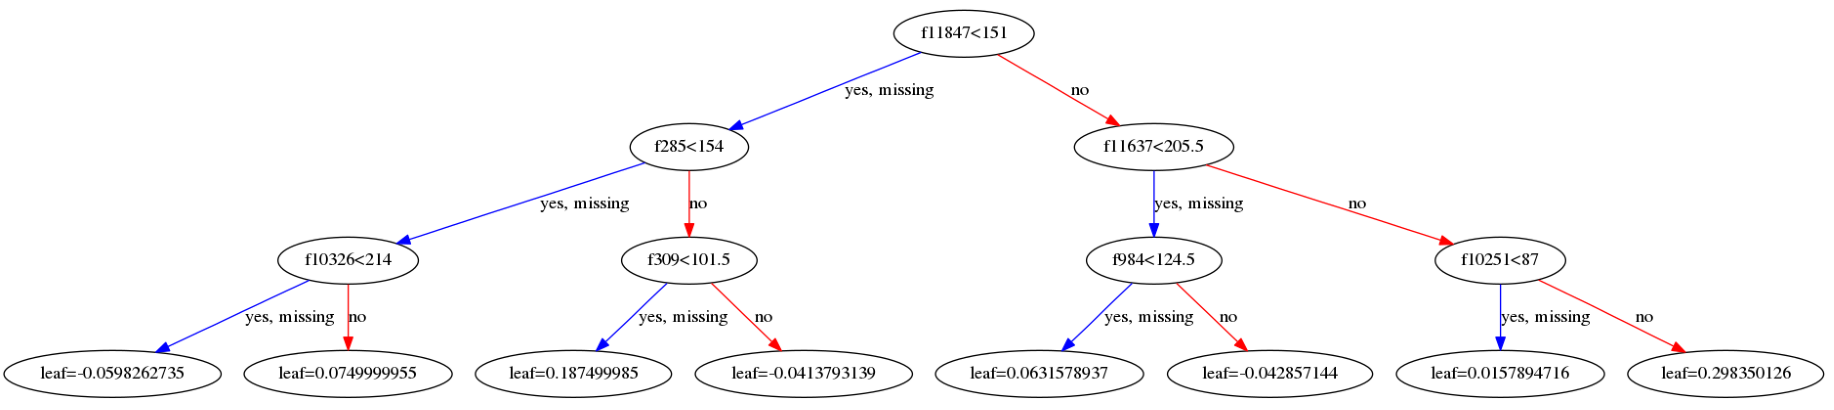
\includegraphics[width=1\textwidth]{images/boosting.png}
		\caption{This is the tree from the boosting model. I have no idea what the numbers or the arrows or the colors or anything mean. It seems like someone plotted this just because it looks good and he would get the bonus points... I would never do that myself.}
		\label{fig:boosting}
	\end{figure}
	\appendix
	\renewcommand\thefigure{\thesection\arabic{figure}} 
	\clearpage   
	\section{Additional Plots}
	\setcounter{figure}{0}    
	\begin{figure}[h]
		\centering
		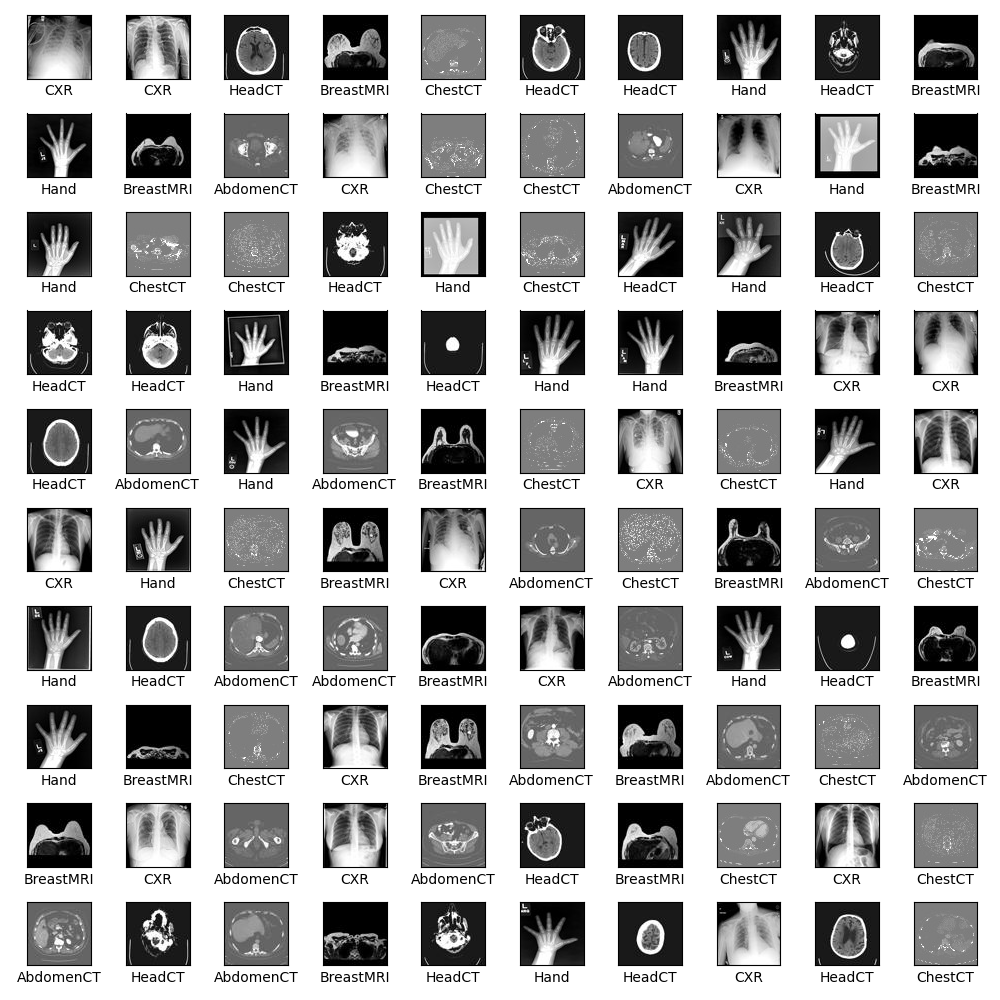
\includegraphics[width=0.8\textwidth]{images/pred_img_cnn.png}
		\caption{The prediction from the convolutional neural network. It misclassified one image. Can you find it?}
		\label{fig:pred_img}
	\end{figure}
	\begin{figure}[h]
		\centering
		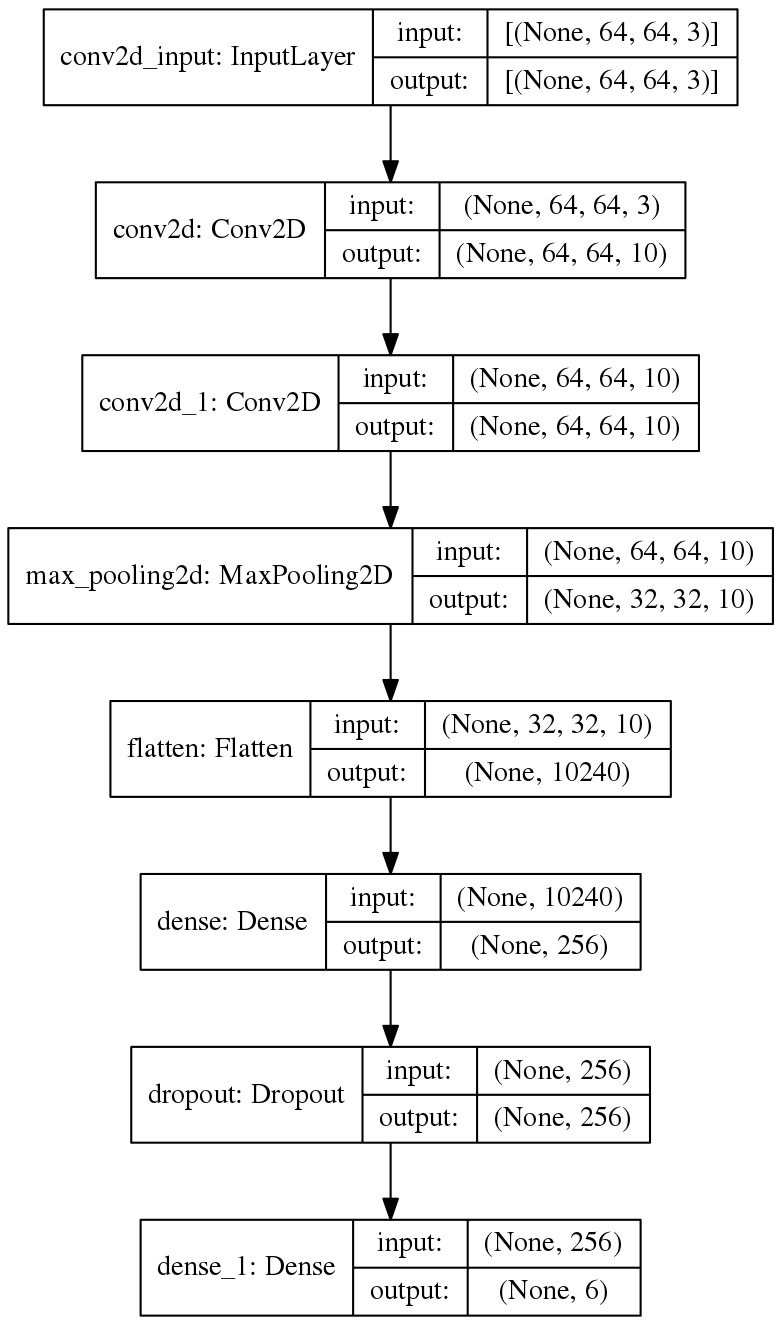
\includegraphics[width=0.3\textwidth]{images/model_cnn.png}
		\caption{The CNN model built with tensorflow.}
		\label{fig:model_cnn}
	\end{figure}
\end{document}